\section{Squidgy Goodness --- more furry friends sightings}
\begin{marginfigure}
\begin{tikzpicture}
\node [name-dest] (box){%
    \begin{minipage}{0.80\textwidth}
     \begin{itemize}
    \item Sam Page
    \item Saber King
    \end{itemize}
    \end{minipage}

};
\node[fancytitle, right=10pt] at (box.north west) {Squidgy Goodness};
\end{tikzpicture}
\end{marginfigure}


Sam 10.50pm: Saber and I headed to \passage{Jericho} today, to continue pushing where Tanguy and I left off last week with a short ~2m drop undescended. The whole of \passage{Jericho} is pretty loose so while Saver contemplated whether or not to continue climbing the rift to reach the pushing front, I set off to drop the undescended pit.
I decided to use a sling around a natural and descended. The natural is dodge and should not be particularly twisted. The drop is fine as a free climb both ways, though it is nice to clip in. At the bottom of this drop, is an unidentified slimy, mouldy wet lump of organic matter like this: 

\bignote{Could this be a dead cave creature, the same type individual as the one I saw last year?}
We could identify furs/hairs, it was covered in slimy mould and water droplets. We both gave it a poke. Whatever it is, its presence is curious in previously unpushed passage. Someone should go take photo/sample.
From here the cave passage continued onwards and upwards, stair like as the rest of \passage{Jericho}. After ~30m, this ended with what would be a climb up, but the sides were quite smooth. Perhaps someone could free climb, but I imagine bolting is required. The passage visibly continues above this climb, plus further climbing up the side of the wall. We surveyed back from here to  the top of the first pit, which was very easy going, if cold  - this passage is extremely draughty- the strongest I have encountered. Our passage is called \passage{Squidgy Goodness}  after both the slimy organic matter and our trip’s reliance on Sorren malt loaf, with its promises of ‘squidgy power’ and ‘squidgy energy’ . As with Tanguy, hot soup in \passage{Sic Semper Tyrannis} was most pleasant.
Getting back to camp was not too bad; although we were worried early on about reaching our callout. I arrived at camp at 21:00. Our first attempt at cooking was methy, but Saber made a good second batch. Although we both agreed that we were not massively passionate about pushing today, it was a good pushing trip. Pushing a going lead and leaving it to push, plus the added interest of our mysterious slime.
We are heading out tomorrow, for my last 2/3 nights of expo. It’s been good \passage{X-Ray}, I’ll be back next year.

\name{Sam Page}



\begin{figure*}[t!]
\checkoddpage \ifoddpage \forcerectofloat \else \forceversofloat \fi
\begin{tikzpicture}
\node [name-dest] (box){%
    \begin{minipage}{0.95\textwidth}
    \begin{multicols}{2}
    

 Went to \passage{Sic Semper Tyrannis} and didn’t get wet! Sam carried the stuff in order not to make it even slower. We went up a dodgy climb and then down a miniclimb Sam rigged a rope off a rock stuck stuck to the side by mud. The remains of last year’s creature were found at the bottom. It looked like this:


Surveyed the windiest passage I’ve been to. The passage ends in a nasty looking climb. Need to send Slovenians. Left gloves at the bottom of  \passage[pitch]{Milka} for lucky finder. Got back to camp and made some Bitterex flavour noodles, threw them into \passage[pitch]{Zimmer} and ate petrol flavour instead.


\name{Saber King}
\end{multicols}
    \end{minipage}

};
\node[fancytitle, right=10pt] at (box.north west) {Saber's view of the matter - UG logbook extract};
\end{tikzpicture}
\end{figure*}



\begin{pagefigure}
\checkoddpage \ifoddpage \forcerectofloat \else \forceversofloat \fi
\centering
\frame{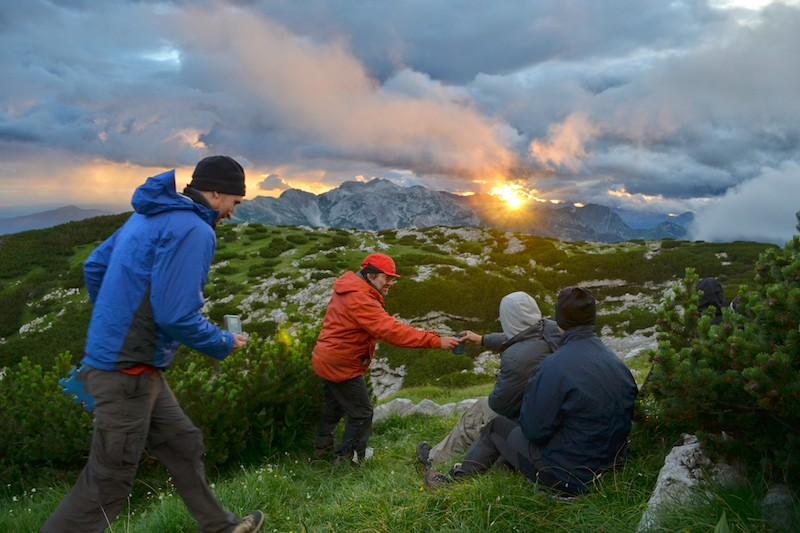
\includegraphics[width=\textwidth]{images/2014/more-extracts-2014/sunset-drinks.jpg}}
\caption{ The back-up sunset spot, sheltered from the winds between rock and dwarf pine still boasts a good view of the mountains --- Rhys Tyers }
\label{SunSet 2014}
\end{pagefigure}
